%%%%%%%%%%%%%%%%%%%%%%%%%%%%%%%%%%%%%%%%%%%%%%%%%%%%%%%%%%%%%%
% CHAPTER 5
%%%%%%%%%%%%%%%%%%%%%%%%%%%%%%%%%%%%%%%%%%%%%%%%%%%%%%%%%%%%%%
\chapter{NLP Pipeline Design}
\label{chap:nlp_pipeline}
\markboth{Chapter \thechapter: NLP Pipeline Design}{}

%%%%%%%%%%%%%%%%%%%%%%%%%%%%%%%%%%%%%%%%%%%%%%%%%%%%%%%%%%%%%%
\section{Introduction}

This chapter presents the proposed Natural Language Processing (NLP) pipeline designed for \textit{DocSaarthi: AI Legal \& Financial Document Assistant}. It describes the overall system architecture, the end-to-end workflow, the feature representation strategy, the model selection strategy, the system requirements, and the proposed evaluation methodology. The design integrates four NLP sub-tasks -- English-to-Hindi machine translation, Legal/Financial document classification, key information extraction, and context-based question answering -- into a single bilingual pipeline, as motivated in Chapter 1 and supported by the research gaps identified in Chapter 2. The design is further grounded in the characteristics of the \textit{DocSaarthi} dataset established through the collection process in Chapter 3 and the preprocessing and exploratory analysis carried out in Chapter 4.

%%%%%%%%%%%%%%%%%%%%%%%%%%%%%%%%%%%%%%%%%%%%%%%%%%%%%%%%%%%%%%
\section{Proposed System Architecture}

The proposed system architecture illustrates the major components of the \textit{DocSaarthi} pipeline, from document acquisition to bilingual response generation.

\begin{figure}[H]
    \centering
    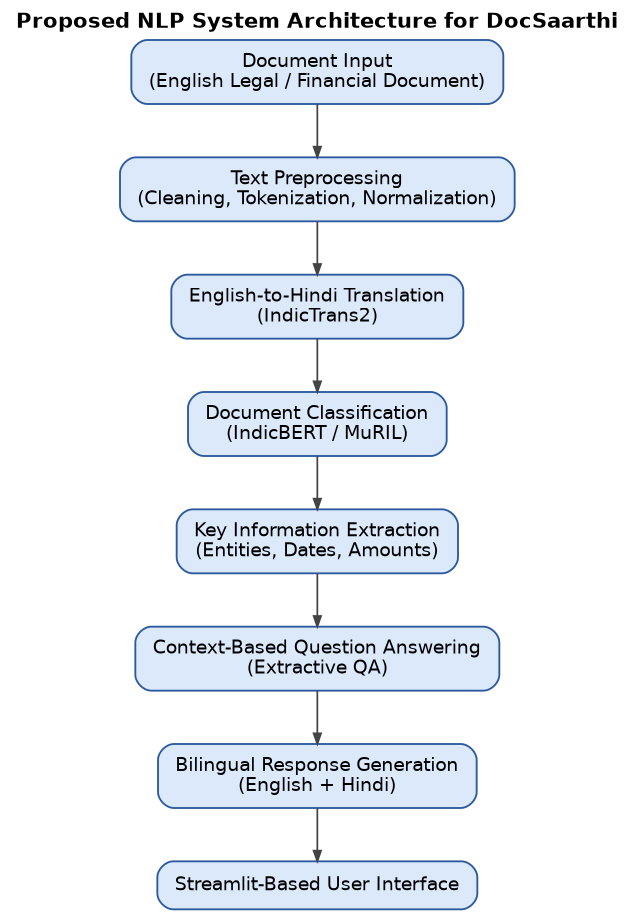
\includegraphics[width=0.95\textwidth]{figures/system_architecture.png}
    \caption{Proposed NLP System Architecture for DocSaarthi}
    \label{fig:system_architecture}
\end{figure}

The architecture consists of the following components:

\begin{enumerate}
    \item \textbf{Document Input:} A user uploads or pastes an English legal or financial document (service agreement, loan contract, insurance policy, tax notice, court proceeding excerpt, or similar) into the system.
    \item \textbf{Text Preprocessing:} The input text undergoes cleaning, tokenization, and normalization, following the preprocessing design established in Chapter 4, so that it is in a suitable form for translation and downstream modelling.
    \item \textbf{English-to-Hindi Translation:} The preprocessed document is translated from English into Hindi using a pre-trained multilingual translation model (IndicTrans2 \cite{gala2023indictrans2}), producing a Hindi version of the document alongside the original English text.
    \item \textbf{Document Classification:} The translated (or original) text is passed to a fine-tuned transformer classifier that assigns a \texttt{Document\_Type} label (Legal or Financial) and a finer-grained \texttt{Intent} label (e.g. Agreement, Loan, Tax), consistent with the label scheme of the \textit{DocSaarthi} dataset described in Chapter 3.
    \item \textbf{Key Information Extraction:} The classified document is scanned for salient fields such as party names, monetary amounts, dates, and durations, using pattern-based rules combined with contextual embeddings from the classification model.
    \item \textbf{Context-Based Question Answering:} A user may pose a natural-language question about the document; an extractive question-answering module locates the answer span within the document text, grounding every response strictly in the uploaded document.
    \item \textbf{Bilingual Response Generation:} The classification result, extracted key information, and question-answering output are rendered to the user in both English and Hindi.
    \item \textbf{Streamlit-Based User Interface:} All of the above stages are exposed to the user through a single interactive Streamlit interface, allowing document upload, translation and classification viewing, and natural-language querying without requiring the user to invoke separate tools.
\end{enumerate}

%%%%%%%%%%%%%%%%%%%%%%%%%%%%%%%%%%%%%%%%%%%%%%%%%%%%%%%%%%%%%%
\section{Workflow Diagram}

Figure~\ref{fig:workflow} illustrates the complete \textit{DocSaarthi} workflow from raw document input to the final bilingual output.

\begin{figure}[H]
    \centering
    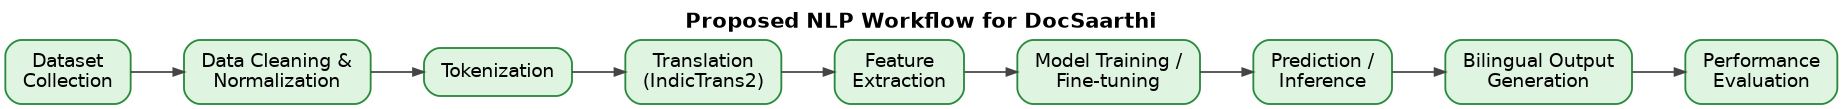
\includegraphics[width=\textwidth]{figures/workflow.png}
    \caption{Proposed NLP Workflow for DocSaarthi}
    \label{fig:workflow}
\end{figure}

The workflow consists of the following stages:

\begin{enumerate}
    \item \textbf{Dataset Collection:} Use of the 400-record, dual-labelled (\texttt{Document\_Type}, \texttt{Intent}) Hindi legal/financial dataset described in Chapter 3 for classification and extraction experiments.
    \item \textbf{Data Cleaning and Normalization:} Unicode and whitespace normalization, as applied to the dataset in Chapter 4.
    \item \textbf{Tokenization:} Word-level tokenization for exploratory analysis and sub-word tokenization for transformer model input.
    \item \textbf{Translation:} English input documents are translated into Hindi using IndicTrans2 prior to, or in parallel with, classification.
    \item \textbf{Feature Extraction:} Contextual sentence and token embeddings are obtained from the selected transformer encoder (Section~\ref{sec:feature_selected}).
    \item \textbf{Model Training / Fine-Tuning:} The classification model is fine-tuned on the labelled \textit{DocSaarthi} dataset; the question-answering module is configured for extractive answer-span prediction over document context.
    \item \textbf{Prediction / Inference:} At inference time, an uploaded document is classified, key information is extracted, and any user question is answered using the document context.
    \item \textbf{Bilingual Output Generation:} Classification labels, extracted fields, and question-answering responses are presented to the user in both English and Hindi.
    \item \textbf{Performance Evaluation:} Each stage is evaluated independently using the metrics defined in Section~\ref{sec:eval_strategy}.
\end{enumerate}

%%%%%%%%%%%%%%%%%%%%%%%%%%%%%%%%%%%%%%%%%%%%%%%%%%%%%%%%%%%%%%
\section{Feature Representation Strategy}

The effectiveness of an NLP model largely depends on how textual information is represented. Various candidate feature extraction techniques, spanning classical count-based methods and modern contextual embeddings, are considered before selecting the most appropriate representation for the bilingual, domain-specific text used in \textit{DocSaarthi}.

\subsection{Candidate Feature Representation Techniques}

\begin{longtable}{|p{4cm}|p{9cm}|}
\hline
\textbf{Technique} & \textbf{Description} \\
\hline
\endfirsthead
\hline
\textbf{Technique} & \textbf{Description} \\
\hline
\endhead
Bag of Words (BoW) & Represents documents using word occurrence counts.\\
\hline
Count Vectorizer & Converts text into frequency vectors.\\
\hline
TF-IDF & Assigns weights based on word importance.\\
\hline
Word2Vec & Dense distributed word embeddings.\\
\hline
GloVe & Global word embedding representation.\\
\hline
FastText & Uses character-level information.\\
\hline
Doc2Vec & Generates document-level embeddings.\\
\hline
BERT & Context-aware transformer embeddings.\\
\hline
RoBERTa & Optimized transformer-based representation.\\
\hline
DistilBERT & Lightweight version of BERT.\\
\hline
IndicBERT & Transformer model for Indian languages.\\
\hline
MuRIL & Multilingual representation for Indian languages.\\
\hline
XLM-R & Cross-lingual multilingual transformer.\\
\hline
\end{longtable}

\subsection{Selected Feature Representation}
\label{sec:feature_selected}

Contextual transformer-based embeddings are selected as the feature representation for \textit{DocSaarthi}, in preference to classical count-based methods (BoW, TF-IDF, Count Vectorizer) and static embeddings (Word2Vec, GloVe, FastText).

\begin{itemize}
    \item \textbf{Selected representation:} Contextual sub-word embeddings produced by an Indian-language-aware transformer encoder (IndicBERT or MuRIL \cite{khanuja2021muril}) for the Hindi classification and extraction stages, and the encoder representations internal to IndicTrans2 \cite{gala2023indictrans2} for the translation stage.
    \item \textbf{Justification:} Static embeddings and count-based representations cannot capture the polysemy and clause-level context that distinguish, for example, a loan agreement clause from a tax clause containing similar vocabulary. Transformer-based contextual embeddings, further pre-trained on Indian-language corpora, are better suited to the code-mixed, template-driven Hindi text identified during the vocabulary analysis in Chapter 4 (Section 4.4).
    \item \textbf{Expected advantages:} Strong out-of-the-box performance on Hindi through Indic-specific pre-training; sub-word tokenization that gracefully handles the limited and repetitive 1,196-word vocabulary of the dataset without excessive out-of-vocabulary issues; transferability from general-domain pre-training to the legal/financial domain through fine-tuning on a relatively small labelled set.
    \item \textbf{Computational requirements:} Fine-tuning a base-sized transformer (110--180M parameters) on the 400-record dataset is feasible on a single consumer-grade GPU or a free-tier cloud GPU runtime, in line with the hardware constraints identified in Chapter 1.
\end{itemize}

%%%%%%%%%%%%%%%%%%%%%%%%%%%%%%%%%%%%%%%%%%%%%%%%%%%%%%%%%%%%%%
\section{Model Selection Strategy}

Different machine learning and deep learning models are considered before selecting the final models for each pipeline stage.

\subsection{Candidate Models}

\begin{longtable}{|p{5cm}|p{8cm}|}
\hline
\textbf{Model} & \textbf{Description} \\
\hline
\endfirsthead
\hline
\textbf{Model} & \textbf{Description} \\
\hline
\endhead
Na\"ive Bayes & Probabilistic classifier.\\
\hline
Logistic Regression & Linear classification model.\\
\hline
Support Vector Machine & Margin-based classifier.\\
\hline
Decision Tree & Tree-based supervised learning model.\\
\hline
Random Forest & Ensemble learning approach.\\
\hline
CNN & Captures local contextual features.\\
\hline
RNN & Sequential learning model.\\
\hline
LSTM & Handles long-term dependencies.\\
\hline
Bi-LSTM & Bidirectional sequential learning.\\
\hline
GRU & Lightweight recurrent model.\\
\hline
Transformer & Attention-based architecture.\\
\hline
BERT & Bidirectional transformer encoder \cite{devlin2019bert}.\\
\hline
IndicBERT & Transformer for Indian languages.\\
\hline
MuRIL & Multilingual Indian language model.\\
\hline
T5 & Text-to-text transformer model.\\
\hline
mT5 & Multilingual T5 model.\\
\hline
IndicTrans2 & Indic-language neural machine translation model.\\
\hline
\end{longtable}

\subsection{Selected Model}

A stage-wise model selection is adopted, since \textit{DocSaarthi} is a multi-task pipeline rather than a single classification problem:

\begin{itemize}
    \item \textbf{Translation stage:} IndicTrans2 \cite{gala2023indictrans2} is selected for English-to-Hindi translation, since it is an open-source model trained specifically for all 22 scheduled Indian languages, including Hindi, and was identified in the literature review (Chapter 2) as the leading available option for this sub-task.
    \item \textbf{Classification stage:} IndicBERT or MuRIL \cite{khanuja2021muril} is selected for the \texttt{Document\_Type} (Legal/Financial) and \texttt{Intent} classification tasks, fine-tuned on the 400-record labelled dataset described in Chapter 3.
    \item \textbf{Key information extraction stage:} The same fine-tuned classification encoder is reused with a token-level (sequence-tagging) head over the extracted entity types (party names, dates, amounts, durations), avoiding the cost of training a separate large model from scratch.
    \item \textbf{Question answering stage:} An extractive question-answering formulation, using a transformer encoder with a span-prediction head over the document context, is selected in preference to a generative approach, so that every answer remains grounded in the source document text.
    \item \textbf{Selection criteria:} Availability of Hindi/Indic pre-training, open-source licensing, feasibility of fine-tuning within the hardware constraints of the micro project, and compatibility with the 400-record dataset size.
    \item \textbf{Advantages:} Reuse of pre-trained Indic language models substantially reduces the data and compute required compared to training from scratch; a shared encoder across classification and extraction reduces pipeline complexity.
    \item \textbf{Expected performance:} Given the dataset's balanced \texttt{Document\_Type} split and template-driven, low-vocabulary-diversity text (Chapter 4), high classification accuracy is expected; translation and question-answering performance is expected to be more sensitive to the fluency of the underlying pre-trained models on domain-specific legal/financial phrasing.
    \item \textbf{Possible limitations:} The 400-record dataset is small relative to typical transformer fine-tuning corpora, the four Financial intent sub-classes are comparatively under-represented (Chapter 4, Section 4.3), and none of the selected models are pre-trained specifically on Indian legal or financial text, which may limit their handling of domain-specific terminology.
\end{itemize}

%%%%%%%%%%%%%%%%%%%%%%%%%%%%%%%%%%%%%%%%%%%%%%%%%%%%%%%%%%%%%%
\section{System Requirements}

\subsection{Hardware Requirements}

\begin{table}[H]
\centering
\caption{Hardware Requirements}
\begin{tabular}{|p{5cm}|p{8cm}|}
\hline
Processor & Intel Core i5 (10th generation or later) / equivalent, quad-core, 2.5 GHz or above\\
\hline
RAM & 8 GB minimum; 16 GB recommended for transformer fine-tuning\\
\hline
Storage & At least 10 GB of free disk space for the dataset, pre-trained model checkpoints (IndicTrans2, IndicBERT/MuRIL), and supporting libraries\\
\hline
GPU (if required) & NVIDIA GPU with 6 GB or more VRAM recommended for fine-tuning; a free-tier cloud GPU runtime (e.g. Google Colab, Kaggle Notebooks) may be used as a substitute when local GPU hardware is unavailable\\
\hline
Internet Connectivity & Required for downloading pre-trained models (IndicTrans2, IndicBERT, MuRIL) and Python packages\\
\hline
\end{tabular}
\end{table}

\subsection{Software Requirements}

\begin{table}[H]
\centering
\caption{Software Requirements}
\begin{tabular}{|p{5cm}|p{8cm}|}
\hline
Operating System & Windows 10/11, Ubuntu 20.04 or later, or equivalent\\
\hline
Programming Language & Python 3.9 or later\\
\hline
IDE & Jupyter Notebook / VS Code / Google Colab\\
\hline
Libraries & pandas, NumPy, Matplotlib/Seaborn (EDA, per Chapter 4); NLTK, Indic NLP Library (preprocessing); HuggingFace Transformers, PyTorch (classification, extraction, question answering); IndicTrans2 toolkit (translation); Streamlit (user interface)\\
\hline
Version Control & Git / GitHub\\
\hline
\end{tabular}
\end{table}

%%%%%%%%%%%%%%%%%%%%%%%%%%%%%%%%%%%%%%%%%%%%%%%%%%%%%%%%%%%%%%
\section{Proposed Evaluation Strategy}
\label{sec:eval_strategy}

\subsection{Automatic Evaluation}

Since \textit{DocSaarthi} integrates four distinct NLP sub-tasks, each pipeline stage is evaluated independently using metrics appropriate to that sub-task.

\begin{longtable}{|p{5.5cm}|p{7.5cm}|}
\hline
\textbf{Pipeline Stage} & \textbf{Evaluation Metrics} \\
\hline
\endfirsthead
\hline
\textbf{Pipeline Stage} & \textbf{Evaluation Metrics} \\
\hline
\endhead
English-to-Hindi Translation & BLEU, chrF++\\
\hline
Document Classification (Legal/Financial, Intent) & Accuracy, Precision, Recall, F1-score\\
\hline
Key Information Extraction & Entity-level Precision, Recall, F1-score\\
\hline
Context-Based Question Answering & Exact Match (EM), F1-score\\
\hline
\end{longtable}

Given the moderate Intent class imbalance observed in Chapter 4 (Section 4.3), macro-averaged Precision, Recall, and F1-score are reported for the classification stage in addition to overall accuracy, so that performance on the less frequent Financial intent sub-classes is not obscured by the majority classes.

\subsection{Human Evaluation}

\begin{itemize}
    \item \textbf{Number of evaluators:} Two to three evaluators (peers and/or faculty guide), sufficient for a semester-long micro project.
    \item \textbf{Evaluation criteria:} Fluency, correctness, relevance, adequacy, coherence, and script correctness of the Hindi output.
    \item \textbf{Rating scale:} A 5-point Likert scale (1 = poor to 5 = excellent) applied per criterion.
    \item \textbf{Evaluation procedure:} A random sample of translation outputs and question-answering responses is reviewed by evaluators without access to the automatic metric scores, to avoid anchoring bias.
    \item \textbf{Agreement method (optional):} Percentage agreement between evaluators is reported where more than one evaluator rates the same sample.
\end{itemize}

\section{Proposed and Implemented Pipeline}

The initial proposal considered transformer-based translation, classification, extraction, and question answering. The implemented Review 3 prototype adopts a lighter architecture: \texttt{pdfjs-dist} for page-level PDF extraction, Unicode-aware preprocessing, lexical Legal/Financial classification, pattern-based information extraction, chunk and token-based retrieval, a 400-record Hindi intent reference set, an offline English-Hindi translation memory, and source-grounded answer generation. OpenAI-based enhancement is optional and disabled by default.

This implementation preserves the project objective while reducing infrastructure cost and hallucination risk. The uploaded PDF remains the only primary source for document facts; the intent dataset and translation memory support routing and language presentation but never replace document evidence.

Suggested evaluation criteria specific to the bilingual nature of \textit{DocSaarthi}:

\begin{itemize}
\item Fluency of the Hindi translation
\item Correctness of the classification label with respect to document content
\item Relevance of the extracted key information to the document
\item Adequacy and groundedness of question-answering responses in the source document
\item Coherence of the bilingual (English and Hindi) response presentation
\item Readability for a non-expert user
\item Script correctness (Devanagari rendering) of Hindi output
\item Cultural and domain appropriateness of legal/financial terminology used
\end{itemize}

%%%%%%%%%%%%%%%%%%%%%%%%%%%%%%%%%%%%%%%%%%%%%%%%%%%%%%%%%%%%%%
\section*{Chapter Summary}

This chapter presented the proposed NLP pipeline for \textit{DocSaarthi}, comprising a system architecture and workflow that carry an English legal or financial document through preprocessing, English-to-Hindi translation (IndicTrans2), document classification and key information extraction (IndicBERT/MuRIL), context-based question answering, and bilingual response generation, exposed to the user through a Streamlit-based interface. Contextual transformer-based embeddings were selected as the feature representation strategy, and a stage-wise model selection approach was adopted across the four pipeline sub-tasks. Hardware and software requirements were defined, and an evaluation strategy combining automatic metrics (BLEU/chrF++, Accuracy/F1, Entity-F1, EM/F1) with structured human evaluation was proposed for each stage. These design decisions provide the foundation for implementing and evaluating the proposed \textit{DocSaarthi} pipeline in subsequent project stages.
